<!DOCTYPE html
    PUBLIC "-//W3C//DTD XHTML 1.0 Strict//EN"
    "http://www.w3.org/TR/xhtml1/DTD/xhtml1-strict.dtd">
<html xmlns="http://www.w3.org/1999/xhtml" lang="en" xml:lang="en">
<head>
 <title>/docs/trunk/english_us/user_guide/core_plugins.tex - Quantum GIS - Trac</title><link rel="start" href="/qgis/wiki" /><link rel="search" href="/qgis/search" /><link rel="help" href="/qgis/wiki/TracGuide" /><link rel="stylesheet" href="/qgis/chrome/common/css/trac.css" type="text/css" /><link rel="stylesheet" href="/qgis/chrome/common/css/code.css" type="text/css" /><link rel="stylesheet" href="/qgis/chrome/common/css/browser.css" type="text/css" /><link rel="icon" href="/favicon.ico" type="image/x-icon" /><link rel="shortcut icon" href="/favicon.ico" type="image/x-icon" /><link rel="up" href="/qgis/browser/docs/trunk/english_us/user_guide?rev=10157" title="Parent directory" /><link rel="alternate" href="/qgis/browser/docs/trunk/english_us/user_guide/core_plugins.tex?rev=10157&amp;format=txt" title="Plain Text" type="text/plain" /><link rel="alternate" href="/qgis/browser/docs/trunk/english_us/user_guide/core_plugins.tex?rev=10157&amp;format=raw" title="Original Format" type="text/x-tex; charset=iso-8859-15" /><style type="text/css">
</style>
 <script type="text/javascript" src="/qgis/chrome/common/js/trac.js"></script>
</head>
<body>


<div id="banner">

<div id="header"><a id="logo" href="http://qgis.org/"><img src="/qgis/chrome/site/qgis-icon.png" width="319" height="102" alt="Quantum GIS" /></a><hr /></div>

<form id="search" action="/qgis/search" method="get">
 <div>
  <label for="proj-search">Search:</label>
  <input type="text" id="proj-search" name="q" size="10" accesskey="f" value="" />
  <input type="submit" value="Search" />
  <input type="hidden" name="wiki" value="on" />
  <input type="hidden" name="changeset" value="on" />
  <input type="hidden" name="ticket" value="on" />
 </div>
</form>



<div id="metanav" class="nav"><ul><li class="first"><a href="/qgis/login">Login</a></li><li><a href="/qgis/settings">Settings</a></li><li><a accesskey="6" href="/qgis/wiki/TracGuide">Help/Guide</a></li><li class="last"><a href="/qgis/about">About Trac</a></li></ul></div>
</div>

<div id="mainnav" class="nav"><ul><li class="first"><a accesskey="1" href="/qgis/wiki">Wiki</a></li><li><a accesskey="2" href="/qgis/timeline">Timeline</a></li><li><a accesskey="3" href="/qgis/roadmap">Roadmap</a></li><li class="active"><a href="/qgis/browser">Browse Source</a></li><li><a href="/qgis/report">View Tickets</a></li><li class="last"><a accesskey="4" href="/qgis/search">Search</a></li></ul></div>
<div id="main">




<div id="ctxtnav" class="nav">
 <ul>
  <li class="first"><a href="/qgis/changeset/9922/docs/trunk/english_us/user_guide/core_plugins.tex">
   Last Change</a></li>
  <li class="last"><a href="/qgis/log/docs/trunk/english_us/user_guide/core_plugins.tex?rev=10157">
   Revision Log</a></li>
 </ul>
</div>


<div id="searchable">
<div id="content" class="browser">
 <h1><a class="first" title="Go to root directory" href="/qgis/browser?rev=10157">root</a><span class="sep">/</span><a title="View docs" href="/qgis/browser/docs?rev=10157">docs</a><span class="sep">/</span><a title="View trunk" href="/qgis/browser/docs/trunk?rev=10157">trunk</a><span class="sep">/</span><a title="View english_us" href="/qgis/browser/docs/trunk/english_us?rev=10157">english_us</a><span class="sep">/</span><a title="View user_guide" href="/qgis/browser/docs/trunk/english_us/user_guide?rev=10157">user_guide</a><span class="sep">/</span><a title="View core_plugins.tex" href="/qgis/browser/docs/trunk/english_us/user_guide/core_plugins.tex?rev=10157">core_plugins.tex</a></h1>

 <div id="jumprev">
  <form action="" method="get">
   <div>
    <label for="rev">View revision:</label>
    <input type="text" id="rev" name="rev" value="10157" size="4" />
   </div>
  </form>
 </div>

 

 
  <table id="info" summary="Revision info"><tr>
    <th scope="col">
     Revision <a href="/qgis/changeset/9922">9922</a>, 3.6 kB
     (checked in by dassau, 1 month ago)
    </th></tr><tr>
    <td class="message"><p>
added qucik print plugin <br />
updated and reviewed gps section <br />
updated external plugin section <br />
</p>
</td>
   </tr><tr>
    <td colspan="2"><ul class="props">
      <li>Property <strong>svn:mergeinfo</strong> set to <em><code></code></em></li>
    </ul></td></tr>
  </table>
  <div id="preview"><table class="code"><thead><tr><th class="lineno">Line</th><th class="content">&nbsp;</th></tr></thead><tbody><tr><th id="L1"><a href="#L1">1</a></th>
<td>% vim: set textwidth=78 autoindent:</td>
</tr><tr><th id="L2"><a href="#L2">2</a></th>
<td></td>
</tr><tr><th id="L3"><a href="#L3">3</a></th>
<td>\section{Uso dei CORE Plugins}\label{sec:core_plugins}\index{plugins!core}</td>
</tr><tr><th id="L4"><a href="#L4">4</a></th>
<td></td>
</tr><tr><th id="L5"><a href="#L5">5</a></th>
<td>% when the revision of a section has been finalized, </td>
</tr><tr><th id="L6"><a href="#L6">6</a></th>
<td>% comment out the following line:</td>
</tr><tr><th id="L7"><a href="#L7">7</a></th>
<td>%\updatedisclaimer</td>
</tr><tr><th id="L8"><a href="#L8">8</a></th>
<td></td>
</tr><tr><th id="L9"><a href="#L9">9</a></th>
<td>QGIS contiene al momento 17 plugins core che possono essere caricati usando la Gestione Plugins.</td>
</tr><tr><th id="L10"><a href="#L10">10</a></th>
<td>La tabella \ref{tab:core_plugins} elenca i plugins CORE e fornisce una  a</td>
</tr><tr><th id="L11"><a href="#L11">11</a></th>
<td>descrizione delle loro funzioni, oltre a mostrare la a loro icona sulla barra degli strumenti. \footnote{The MapServer</td>
</tr><tr><th id="L12"><a href="#L12">12</a></th>
<td>Export Plugin e Plugin Installer sono plugins esterni Python,</td>
</tr><tr><th id="L13"><a href="#L13">13</a></th>
<td>ma fanno parte della sorgente QGIS e automaticamente caricati e selezionabili </td>
</tr><tr><th id="L14"><a href="#L14">14</a></th>
<td>dal Gestore dei Plugins.}</td>
</tr><tr><th id="L15"><a href="#L15">15</a></th>
<td></td>
</tr><tr><th id="L16"><a href="#L16">16</a></th>
<td>% minipage is needed to appear the footnote under the table</td>
</tr><tr><th id="L17"><a href="#L17">17</a></th>
<td>% SH</td>
</tr><tr><th id="L18"><a href="#L18">18</a></th>
<td>\begin{minipage}{\textwidth}</td>
</tr><tr><th id="L19"><a href="#L19">19</a></th>
<td>\begin{table}[H]</td>
</tr><tr><th id="L20"><a href="#L20">20</a></th>
<td>\centering</td>
</tr><tr><th id="L21"><a href="#L21">21</a></th>
<td>\caption{QGIS Core Plugins}\label{tab:core_plugins}\medskip</td>
</tr><tr><th id="L22"><a href="#L22">22</a></th>
<td>\small</td>
</tr><tr><th id="L23"><a href="#L23">23</a></th>
<td>&nbsp;\begin{tabular}{|l|l|p{4in}|}</td>
</tr><tr><th id="L24"><a href="#L24">24</a></th>
<td>\hline \textbf{Icona} &amp; \textbf{Plugin} &amp; \textbf{Descrizione}\\</td>
</tr><tr><th id="L25"><a href="#L25">25</a></th>
<td>\hline</td>
</tr><tr><th id="L26"><a href="#L26">26</a></th>
<td>
\includegraphics[width=0.6cm]{delimited_text}</td>
</tr><tr><th id="L27"><a href="#L27">27</a></th>
<td>&nbsp;&amp; Aggiungi layer testo delimitato \index{plugins!delimited text} &amp; Carica e mostra files di testo delimitato contnenti coordinate x,y\\</td>
</tr><tr><th id="L28"><a href="#L28">28</a></th>
<td>\hline</td>
</tr><tr><th id="L29"><a href="#L29">29</a></th>
<td>
\includegraphics[width=0.6cm]{coordinate_capture}</td>
</tr><tr><th id="L30"><a href="#L30">30</a></th>
<td>&nbsp;&amp; Cattura coordinate \index{plugins!coordinate capture}&amp; Cattura le coordinate del mouse in un diverso SRS\\</td>
</tr><tr><th id="L31"><a href="#L31">31</a></th>
<td>\hline </td>
</tr><tr><th id="L32"><a href="#L32">32</a></th>
<td>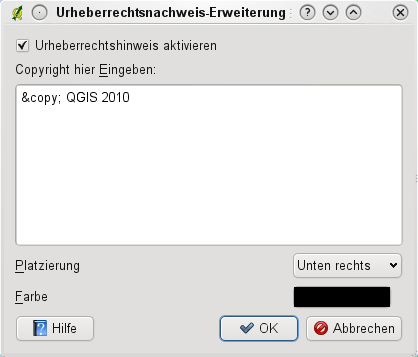
\includegraphics[width=0.6cm]{copyright_label}</td>
</tr><tr><th id="L33"><a href="#L33">33</a></th>
<td>&nbsp;&amp; Etichetta di Copyright \index{plugins!copyright}&amp; Stampa le informazioni di copyright\\</td>
</tr><tr><th id="L34"><a href="#L34">34</a></th>
<td>\hline </td>
</tr><tr><th id="L35"><a href="#L35">35</a></th>
<td>
\includegraphics[width=0.6cm]{dxf2shp_converter}</td>
</tr><tr><th id="L36"><a href="#L36">36</a></th>
<td>&nbsp;&amp; Convertitore DXF2Shp \index{plugins!DXF2Shape}&amp; Converte files da formato DXF a SHP\\</td>
</tr><tr><th id="L37"><a href="#L37">37</a></th>
<td>\hline</td>
</tr><tr><th id="L38"><a href="#L38">38</a></th>
<td>
\includegraphics[width=0.6cm]{gps_importer}</td>
</tr><tr><th id="L39"><a href="#L39">39</a></th>
<td>&nbsp;&amp; Strumenti GPS \index{plugins!gps}&amp; Strumenti per caricare e importare dati GPS\\</td>
</tr><tr><th id="L40"><a href="#L40">40</a></th>
<td>\hline</td>
</tr><tr><th id="L41"><a href="#L41">41</a></th>
<td>
\includegraphics[width=0.6cm]{grass}</td>
</tr><tr><th id="L42"><a href="#L42">42</a></th>
<td>&nbsp;&amp; GRASS \index{plugin!grass toolbox} &amp; Attiva il potente strumentario GRASS\\</td>
</tr><tr><th id="L43"><a href="#L43">43</a></th>
<td>\hline</td>
</tr><tr><th id="L44"><a href="#L44">44</a></th>
<td>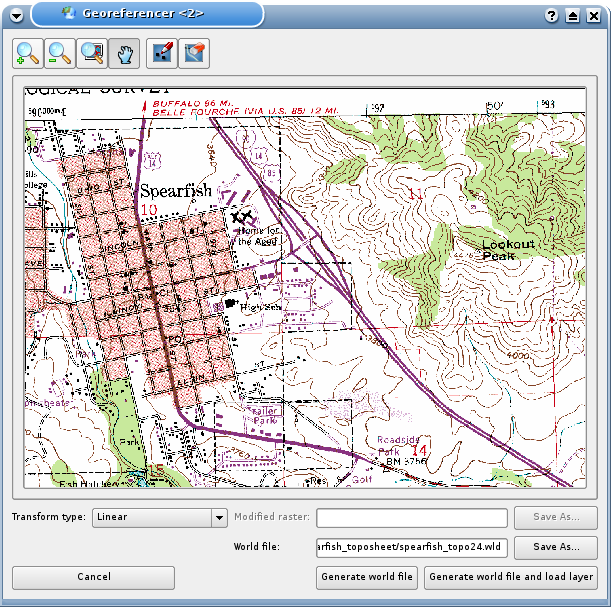
\includegraphics[width=0.6cm]{georeferencer}</td>
</tr><tr><th id="L45"><a href="#L45">45</a></th>
<td>&nbsp;&amp; Georeferenziatore \index{plugin!georeferencer} &amp; Aggiunge le informazioni di proiezione nei raster\\</td>
</tr><tr><th id="L46"><a href="#L46">46</a></th>
<td>\hline</td>
</tr><tr><th id="L47"><a href="#L47">47</a></th>
<td>
\includegraphics[width=0.6cm]{grid_maker}</td>
</tr><tr><th id="L48"><a href="#L48">48</a></th>
<td>&nbsp;&amp; Generatore di griglia \index{plugins!graticule}&amp; Genera una griglia latitude/longitude e la salva come file shape\\</td>
</tr><tr><th id="L49"><a href="#L49">49</a></th>
<td>\hline</td>
</tr><tr><th id="L50"><a href="#L50">50</a></th>
<td>
\includegraphics[width=0.6cm]{interpolation}</td>
</tr><tr><th id="L51"><a href="#L51">51</a></th>
<td>&amp; Plugin di Interpolazione \index{plugins!Interpolation}&amp; Plugin per l'interpolazione basata sui vertici di un layer vettoriale\\</td>
</tr><tr><th id="L52"><a href="#L52">52</a></th>
<td>\hline</td>
</tr><tr><th id="L53"><a href="#L53">53</a></th>
<td>
\includegraphics[width=0.6cm]{mapserver_export}</td>
</tr><tr><th id="L54"><a href="#L54">54</a></th>
<td>&amp; MapServer Export \index{plugins!MapServer Export}&amp; Esporta e salva un file di progetto QGIS in un file di mappa Mapserver \\</td>
</tr><tr><th id="L55"><a href="#L55">55</a></th>
<td>\hline</td>
</tr><tr><th id="L56"><a href="#L56">56</a></th>
<td>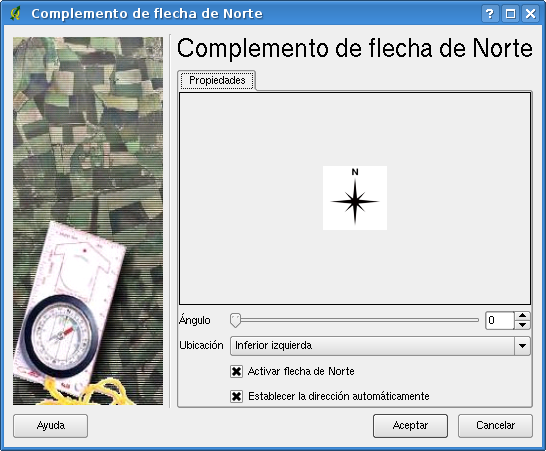
\includegraphics[width=0.6cm]{north_arrow}</td>
</tr><tr><th id="L57"><a href="#L57">57</a></th>
<td>&amp; Freccia Nord \index{plugins!north arrow}&amp; Mostra una freccia orientata a nord sovrapposta alla pagina\\</td>
</tr><tr><th id="L58"><a href="#L58">58</a></th>
<td>\hline</td>
</tr><tr><th id="L59"><a href="#L59">59</a></th>
<td>
\includegraphics[width=0.6cm]{ogr_converter}</td>
</tr><tr><th id="L60"><a href="#L60">60</a></th>
<td>&nbsp;&amp; Convertitore Layer OGR \index{plugins!OGR converter} &amp; Converte layer</td>
</tr><tr><th id="L61"><a href="#L61">61</a></th>
<td>vettoriali fra i formati supportati dalla libreria OGR\\</td>
</tr><tr><th id="L62"><a href="#L62">62</a></th>
<td>\hline</td>
</tr><tr><th id="L63"><a href="#L63">63</a></th>
<td>
\includegraphics[width=0.6cm]{plugin_installer}</td>
</tr><tr><th id="L64"><a href="#L64">64</a></th>
<td>&nbsp;&amp; Istallatore di Plugin \index{plugins!Plugin Installer} &amp; Scarica e istalla Plugin Python di QGIS\\</td>
</tr><tr><th id="L65"><a href="#L65">65</a></th>
<td>\hline</td>
</tr><tr><th id="L66"><a href="#L66">66</a></th>
<td>
\includegraphics[width=0.6cm]{spiticon}</td>
</tr><tr><th id="L67"><a href="#L67">67</a></th>
<td>&nbsp;&amp; SPIT \index{plugins!spit}&amp; Strumento per importare file shape in PostgreSQL/PostGIS \\</td>
</tr><tr><th id="L68"><a href="#L68">68</a></th>
<td>\hline</td>
</tr><tr><th id="L69"><a href="#L69">69</a></th>
<td>
\includegraphics[width=0.6cm]{quick_print}</td>
</tr><tr><th id="L70"><a href="#L70">70</a></th>
<td>&nbsp;&amp; Quick Print \index{plugins!quick print}&amp; Stampa rapidamente una mappa col minimo sforzo</td>
</tr><tr><th id="L71"><a href="#L71">71</a></th>
<td>effort \\</td>
</tr><tr><th id="L72"><a href="#L72">72</a></th>
<td>\hline</td>
</tr><tr><th id="L73"><a href="#L73">73</a></th>
<td>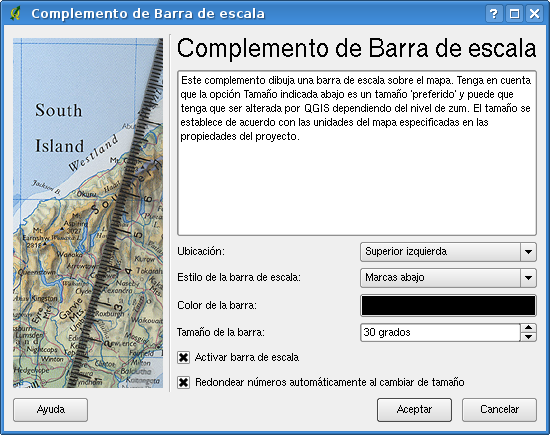
\includegraphics[width=0.6cm]{scale_bar}</td>
</tr><tr><th id="L74"><a href="#L74">74</a></th>
<td>&nbsp;&amp; Barra di scala \index{plugins!scalebar}&amp; Genera una barra di scala\\</td>
</tr><tr><th id="L75"><a href="#L75">75</a></th>
<td>\hline</td>
</tr><tr><th id="L76"><a href="#L76">76</a></th>
<td>
\includegraphics[width=0.6cm]{mIconAddWfsLayer}</td>
</tr><tr><th id="L77"><a href="#L77">77</a></th>
<td>&nbsp;&amp; WFS &amp; Load and display WFS layer \\</td>
</tr><tr><th id="L78"><a href="#L78">78</a></th>
<td>\hline</td>
</tr><tr><th id="L79"><a href="#L79">79</a></th>
<td>\end{tabular}</td>
</tr><tr><th id="L80"><a href="#L80">80</a></th>
<td>\end{table}</td>
</tr><tr><th id="L81"><a href="#L81">81</a></th>
<td>\end{minipage}</td>
</tr><tr><th id="L82"><a href="#L82">82</a></th>
<td></td>
</tr><tr><th id="L83"><a href="#L83">83</a></th>
<td>\normalsize</td>
</tr><tr><th id="L84"><a href="#L84">84</a></th>
<td></td>
</tr><tr><th id="L85"><a href="#L85">85</a></th>
<td>\begin{Tip}\caption{\textsc{Settaggio dei Plugins salvati in un progetto}}\index{plugins settings}</td>
</tr><tr><th id="L86"><a href="#L86">86</a></th>
<td>\qgistip{Quando si salva un progetto di QGIS ogni modifica fatta sui plugins Freccia del Nord, Barra di scala 
Etichetta di copyrigth saranno salvate nel progetto e ricaricate al prossimo uso del progetto.}</td>
</tr><tr><th id="L87"><a href="#L87">87</a></th>
<td>\end{Tip}</td>
</tr></tbody></table>
  </div>

 <div id="help">
  <strong>Note:</strong> See <a href="/qgis/wiki/TracBrowser">TracBrowser</a> for help on using the browser.
 </div>

  <div id="anydiff">
   <form action="/qgis/anydiff" method="get">
    <div class="buttons">
     <input type="hidden" name="new_path" value="/docs/trunk/english_us/user_guide/core_plugins.tex" />
     <input type="hidden" name="old_path" value="/docs/trunk/english_us/user_guide/core_plugins.tex" />
     <input type="hidden" name="new_rev" value="10157" />
     <input type="hidden" name="old_rev" value="10157" />
     <input type="submit" value="View changes..." title="Prepare an Arbitrary Diff" />
    </div>
   </form>
  </div>

</div>
</div>
<script type="text/javascript">searchHighlight()</script>
<div id="altlinks"><h3>Download in other formats:</h3><ul><li class="first"><a href="/qgis/browser/docs/trunk/english_us/user_guide/core_plugins.tex?rev=10157&amp;format=txt">Plain Text</a></li><li class="last"><a href="/qgis/browser/docs/trunk/english_us/user_guide/core_plugins.tex?rev=10157&amp;format=raw">Original Format</a></li></ul></div>

</div>

<div id="footer">
 <hr />
 <a id="tracpowered" href="http://trac.edgewall.org/"><img src="/qgis/chrome/common/trac_logo_mini.png" height="30" width="107"
   alt="Trac Powered"/></a>
 <p class="left">
  Powered by <a href="/qgis/about"><strong>Trac 0.10.3.1</strong></a><br />
  By <a href="http://www.edgewall.org/">Edgewall Software</a>.
 </p>
 <p class="right">
  Visit the Quantum GIS open source project at<br /><a href="http://qgis.org">http://qgis.org/</a>
 </p>
</div>



 </body>
</html>

